\documentclass{article}
\usepackage{pgfplots}
\usepackage[paperwidth=7.8cm,paperheight=6.1cm,left=0cm,right=0cm,top=0cm,bottom=0cm]{geometry}
\pgfplotsset{compat=1.18, width = 8cm}
\pagestyle{empty}
\begin{document}
\begin{center}
  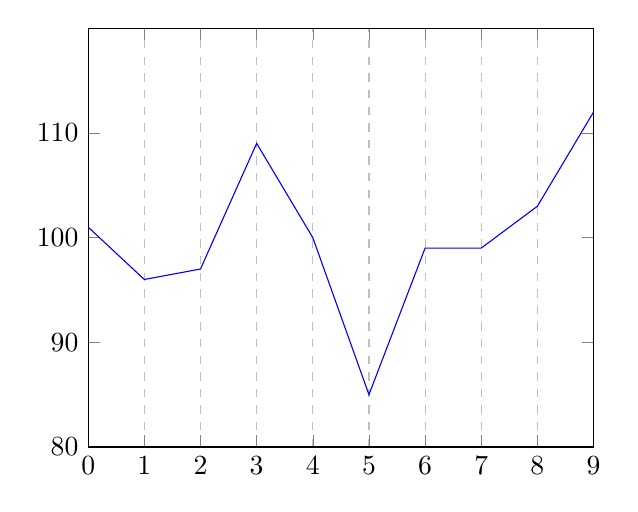
\begin{tikzpicture}
    \begin{axis}[
      xmin=0, xmax=9,
      ymin=80, ymax=120,
      xtick={0,1,2,3,4,5,6,7,8,9},
      ytick={80,90,100,110},
      xmajorgrids=true,
      grid style=dashed,
      ]
      \addplot[
        color=blue,
        ]
        coordinates{
        (0, 101)(1, 96)(2, 97)(3, 109)(4, 100)(5, 85)(6, 99)(7, 99)(8, 103)(9, 112)};
      \end{axis} 
    \end{tikzpicture}  
  \end{center}
  \end{document}
